\chapter{Preliminaries}
\label{chp:chapter2}
\graphicspath{{figures/}{figures/chapter2/}}
\pgfplotsset{
    table/search path={{figures/chapter2/data},{data}},
}

Isogeometric analysis (IGA), introduced by Hughes et al. \cite{HUGHES20054135}, adopts the spline basis, which underlies the CAD geometry, as the basis for analysis. Of particular importance is the positive impact of smoothness on numerical solutions, where, in many application domains, IGA outperforms classical finite elements~\cite{cottrell2009isogeometric,cottrell_studies_2007,cottrell2006isogeometric,hughes_duality_2008,bazilevs_isogeometric_2010,evans_n-widths_2009}.

In this chapter, a brief overview of spline basis functions that are most commonly used in Isogeometric Analysis are given in~\ref{sec:spline_overview}. In~\ref{sec:geometric_algorithms}, we review some of the most popular algorithms in manipulating splines including \Bezier extraction and \Bezier projection. Dual basis serves as the main research tool for this thesis. The concept of dual basis functions is also introduced in~\ref{sec:dual_basis}.

\section{Splines}\label{sec:spline_overview}

\subsection{The univariate Bernstein basis}

The $i^{\text{th}}$ univariate Bernstein basis function of degree $p$ on the unit interval $\left[ 0,1 \right]$ is defined by
\begin{equation}
    B_i^p(\xi) = \binom {p}{i}\xi^i(1-\xi)^{p-i}
\end{equation}
where the binomial coefficient $\binom {p}{i}=\dfrac{p!}{i!(p-i)!}$, $0\leq{i}\leq{p}$. The polynomial degree superscript will be omitted when unnecessary. Matrix-vector notation will be used throughout, with bold fonts indicating matrices and vectors, e.g. the vector form of a set of Bernstein basis functions is denoted by
\begin{equation}
    \mathbf{B}^p(\xi)=
    \begin{bmatrix}
        B_0^p(\xi) \\
        B_1^p(\xi) \\
        \vdots     \\
        B_p^p(\xi)
    \end{bmatrix}.
\end{equation}
The Bernstein basis of degree $p$ spans the space of polynomials of degree $p$. The Gramian matrix $\mathbf{G}^p = [G_{i,j}^p]$ can be computed by
\begin{equation}
    G_{i,j}^p=\int_0^1B_i^p(\xi) B_j^p(\xi)d\xi,\qquad{i,j\in\left\{0,1,\dots, p\right\}}.\label{eq:gramian_bernstein}
\end{equation}
Eq.~\eqref{eq:gramian_bernstein} can be evaluated in closed form (see~\cite{farouki1988algorithms}) as
\begin{equation}
    G_{i,j}^p = \frac{\binom {p}{i}\binom {p}{j}}{(2p+1)\binom {2p}{i+j}}\label{eq:gramian_bernstein_closed_form}
\end{equation}
and its inverse (see~\cite{juttler1998dual}) as
\begin{equation}
    [G_{i,j}^p]^{-1} = \frac{(-1)^{i+j}}{\binom {p}{i}\binom {p}{j}}\sum_{k=0}^{\min(i,j)}\binom{p+k+1}{p-i}\binom{p-k}{p-i}\binom{p+k+1}{p-j}\binom{p-k}{p-j}.\label{eq:inverse_gramian_bernstein_closed_form}
\end{equation}
A Bernstein basis defined over an arbitrary interval $\left[\xi_\alpha,\xi_\beta\right]$ can be evaluated from
\begin{equation}
    B_i^p(\frac{\xi-\xi_\alpha}{\xi_\beta-\xi_\alpha}),\qquad \xi\in\left[\xi_\alpha,\xi_\beta\right].
\end{equation}
The corresponding Gramian and inverse can be obtained by multiplying and dividing the matrices in Eq.~\eqref{eq:gramian_bernstein_closed_form} and Eq.~\eqref{eq:inverse_gramian_bernstein_closed_form} by the scaling factor $(\xi_\beta-\xi_\alpha)$, respectively. For the sake of simplicity, we use the same symbols to represent the Bernstein basis defined on different intervals. A closed form expression for the $L^2$ inner product between the Bernstein basis $B_i^p(\xi)$ and polynomial $\xi^j$ is given by
\begin{equation}
    \int_0^1 B_i^p (\xi) \xi^j d\xi = \binom{p}{i} \frac{(i+j)! (p-i)!}{(p+j+1)!}.\label{eq:inner_product_bernstein_polynomial}
\end{equation}

Bernstein basis possess the following properties:
\begin{itemize}
    \item Nonnegativity: $B_i^p(\xi)\geq 0$ for all $i$, $p$, and $0\leq\xi\leq 1$;
    \item Partition of unity: $\sum_{i=0}^pB_i^p(\xi)=1$, for all $0\leq\xi\leq 1$;
    \item Interpolatory at the ends: $B_0^p(0)=B_p^p(1)=1$.
\end{itemize}
% Given a set of control points $\left\{\mathbf{P}_i\right\}_{i=0}^p$, the corresponding \Bezier curve is defined by:
% \begin{equation}
%     \mathbf{C}(\xi) = \sum_{i=1}^p\mathbf{P}_i B_i^p(\xi).
% \end{equation}

However, the global support of the Bernstein basis makes it impossible to locally edit a \Bezier curve, which is a urgent requirement for geometry modeling. This problem can be overcome by using B-splines.

\subsection{The univariate B-spline basis}

A set of univariate B-spline basis functions of degree $p$ can be uniquely defined by a non-decreasing knot vector $\mathbf{\Xi}=\left\{\xi_i\right\}_{i=0}^{n+p}$, where $n$ is the number of B-spline basis functions. In this work, we only use open knot vectors, i.e., $\xi_0=\xi_1=\dots=\xi_{p}$ and $\xi_{n}=\xi_{n+1}=\dots=\xi_{n+p}$ defined over the interval $\left[0,1\right]$. The value of the $i^{\text{th}}$ B-spline basis function is recursively defined using the Cox-de Boor formula~\cite{piegl2012nurbs}
\begin{align}
    N_{i}^0(\xi) & =\begin{cases}1 & \xi_i\leq{\xi}\leq{\xi_{i+1}}\\0 & \text{otherwise} \end{cases}                                                                                          \\
    N_{i}^p(\xi) & =\frac{\xi-\xi_i}{\xi_{i+p}-\xi_i}N_{i}^{p-1}(\xi)+\frac{\xi_{i+p+1}-\xi}{\xi_{i+p+1}-\xi_{i+1}}N_{i+1}^{p-1}(\xi).
\end{align}

In addition to the properties of Bernstein basis, B-splines also possess:
\begin{itemize}
    \item Compact support: $\supp{N_{i}^p}\subset \left[\xi_i,\xi_{i+p+1}\right]$.
\end{itemize}
This feature is crucial for both geometry modeling and finite element analysis. In modeling, it allows the changing in a localized region while keeping other parts unchanges. In finite element analysis, it ensures the sparse structure of the discretized linear system.

\begin{figure}[ht]
    \center
    \begin{subfigure}[t]{\linewidth}
        \center
        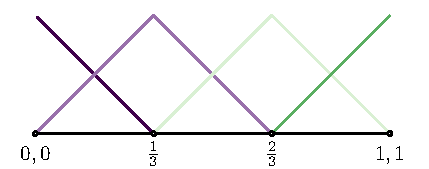
\includegraphics[scale=1.2]{p=1_space}
    \end{subfigure}
    \begin{subfigure}[t]{\linewidth}
        \center
        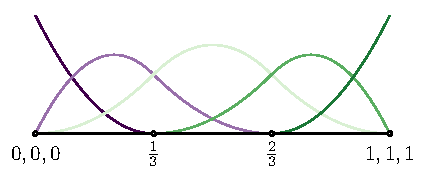
\includegraphics[scale=1.2]{p=2_space}
    \end{subfigure}
    \caption[B-spline basis functions of different degrees.]{B-spline basis functions of different degrees. Top: linear spline basis functions defined by $\left\{0,0,1/3,2/3,1,1\right\}$. Bottom: quadratic spline basis functions defined by $\left\{0,0,0,1/3,2/3,1,1,1\right\}$.}\label{fig:spline_basis}
\end{figure}

B-splines of different degrees are shown in Figure~\ref{fig:spline_basis}. As can be seen, linear B-spline basis functions are identical to the classic hat functions that widely used in finite element analysis. Compared with quadratic Lagrange polynomials in Figure~\ref{fig:lagrange_polynomial}, quadratic B-splines are smoother across each mesh grids. Indeed, B-splines of degree $p$ have up to $p-1$ continuous derivatives. The inter-element continuity can be manipulated by repeating knots. In general, basis functions at knot of multiplicity $m$ are $C^{p-m}$ continuity.

\begin{figure}[ht]
    \center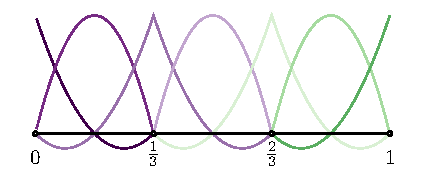
\includegraphics[scale=1.2]{p=2_space_2}
    \caption{Quadratic Lagrange polynomials defined on the same mesh grid as the splines in Figure~\ref{fig:spline_basis}.}\label{fig:lagrange_polynomial}
\end{figure}


A $d$-dimensional B-spline curve $\mathbf{S}(\xi)\in{\R^d}$ can then be defined as
\begin{equation}
    \mathbf{S}(\xi)=\sum_A N_{A,p}(\xi)\mathbf{P}_A
\end{equation}
where $\mathbf{P}_A=(p_A^1,p_A^2,\ldots,p_A^d)^T$ is a $d$-dimensional control point. An example of a B-spline curve is illustrated in Figure~\ref{fig:b-spline_and_geometry}.

\begin{figure}[ht]
    \center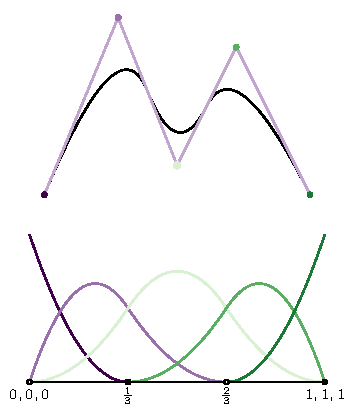
\includegraphics[scale=1.3]{geometry}
    \caption{A B-spline piecewise quadratic curve in $\R^2$ and the corresponding B-spline basis.}\label{fig:b-spline_and_geometry}
\end{figure}

\FloatBarrier
\subsection{The univariate NURBS basis}

B-splines can be used to represent piecewise polynomial functions but are not capable of representing conic sections (e.g. circles, ellipses and hyperbolas). NURBS(Non-Uniform Rational B-Spline) overcome this shortcoming.  A NURBS basis function can be written as
\begin{equation}
    R_{A,p}(\xi)=\dfrac{N_{A,p}(\xi)w_A}{W{(\xi)}}
\end{equation}
where $w_A$ is called a weight and
\begin{align}
    \label{eq:weight}
    W(\xi)=\sum_{A} N_{A,p}(\xi)w_A
\end{align}
is called the weight function. A $d$-dimensional rational curve $\mathbf{S}(\xi)\in{\R^d}$ can then be defined as
\begin{equation}
    \mathbf{S}(\xi)=\sum_A R_{A,p}(\xi)\mathbf{P}_A.
\end{equation}
It is often more convenient to represent the $d$-dimensional NURBS in a $(d+1)$-dimensional homogeneous space by defining $\mathbf{P}_A^w=(p_A^1w_A,p_A^2w_A,\ldots,p_A^dw_A,w_A)^T$ and the corresponding $(d+1)$-dimensional B-spline curve as
\begin{align}
    \mathbf{S}^w(\xi) & =\sum_A N_{A,p}(\xi)\mathbf{P}_A^w
\end{align}
such that each component of $\mathbf{S}^w$ can be written as
\begin{align}
    S_i(\xi) & =\dfrac{{S}_i^w(\xi)}{{S}_{d+1}^w(\xi)}.
\end{align}
In the homogeneous form, NURBS can be manipulated with standard B-spline algorithms.

\subsection{The multivariate spline basis}

In higher dimensions, Bernstein, B-spline, and NURBS basis functions are formed by the Kronecker product of univariate basis functions. For example, two-dimensional B-spline basis functions of degree $\mathbf{p}=(p_\xi, p_\eta)$ are defined by
\begin{equation}
    \mathbf{N}^\mathbf{p}(\xi,\eta)=\mathbf{N}^{p_\xi}(\xi)\otimes\mathbf{N}^{p_\eta}(\eta)
\end{equation}
where $\mathbf{N}^{p_\xi}(\xi)$ and $\mathbf{N}^{p_\eta}(\eta)$ are vectors of basis functions in the $\xi$ and $\eta$ directions, respectively. A particular multivariate basis function can be written as
\begin{equation}
    {N}_{A(i,j)}^\mathbf{p}(\xi,\eta)={N}_{i,p_\xi}(\xi){N}_{j,p_\eta}(\eta)
\end{equation}
where the index mapping is defined as
\begin{equation}
    A(i,j)=n_\eta{i}+j.
\end{equation}
The integer $n_\eta$ is the number of basis functions in $\eta$ direction. In three-dimensional space, a set of basis functions can be constructed by the Kronecker product between two-dimensional basis functions and univariate basis functions.

\section{Geometric Algorithms}\label{sec:geometric_algorithms}

\subsection{Knot insertion}

The knot insertion algorithm ensures the insertion of one or multiple knots into a knot vector $\mathbf{\Xi}$ without changing the shape and parameterization of the curve. It allows us to conduct \textit{h}-refinement (subdividing elements into smaller ones without changing the type of basis functions used) in the context of Isogeometric Analysis. The detailed algorithm of knot insertion can be found in~\cite{piegl2012nurbs}.

An example of knot insertion of the B-spline curve in Figure~\ref{fig:b-spline_and_geometry} is illustrated in Figure~\ref{fig:b-spline_h_refine}. A set of knots $\left\{\frac{1}{6}, \frac{1}{2}, \frac{5}{6}\right\}$ are inserted into the original knot vector $\mathbf{\Xi}=\left\{0,0,0,1/3,2/3,1,1,1\right\}$.  The inserted curve remains geometrically and parametrically identical to the original curve. Meanwhile, knot spans $[ \xi_i,\xi_{i+1} )$ are splitted into smaller ones.

\begin{figure}[ht]
    \center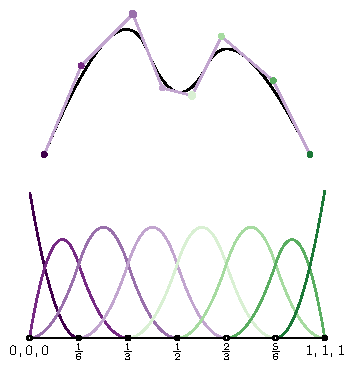
\includegraphics[scale=1.3]{h_refine}
    \caption{Knot insertion for the curve in Figure~\ref{fig:b-spline_and_geometry}. The inserted curve is geometrically and parametrically identical to the original curve.}\label{fig:b-spline_h_refine}
\end{figure}

\subsection{Degree elevation}

The degree elevation algorithm increases the polynomial degree of each B-spline basis functions while preserves the geometry and parameterization of the curve. It allows us to conduct \textit{p}-refinement (increasing the degree of basis functions without changing the number of element used) in the context of Isogemetric Analysis. The detailed algorithm of degree elevation can be found in~\cite{piegl2012nurbs}.

An example of degree elevation of the B-spline curve in Figure~\ref{fig:b-spline_and_geometry} is illustrated in Figure~\ref{fig:b-spline_p_refine}, where the original quadratic spline curve is elevated to cubic and the shape remains unchanged. Recalling that the basis is $C^{p-m}$ continuous at a knot of multiplicity $m$, it is clear that, to preserve the inter-element continuity, the multiplicity of each knots must be increased as the increase of the polynomial degree. In Figure~\ref{fig:b-spline_p_refine}, the multiplicity each knot is increased by one.

\begin{figure}[ht]
    \center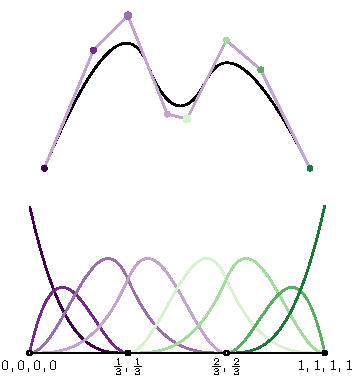
\includegraphics[scale=1.3]{p_refine}
    \caption{Degree elevation for the curve in Figure~\ref{fig:b-spline_and_geometry}. The degree elevated curve is geometrically and parametrically identical to the original curve.}\label{fig:b-spline_p_refine}
\end{figure}

\subsection{\Bezier extration}

\Bezier extraction is a technique that is often used to facilitate the incorporation of isogeometric analysis into existing finite element codes~\cite{borden2011isogeometric,scott2011isogeometric}. \Bezier extraction defines an injection that maps a space spanned by B-spline basis to a space spanned by piecewise Bernstein basis. \Bezier extraction is accomplished by repeating all interior knots of a knot vector until they have a multiplicity equal to $p+1$. The interior knots repeating process defines a linear operator $\mathbf{C}$ (see~\cite{borden2011isogeometric}) such that
\begin{equation}
    \mathbf{N}(\xi)=\mathbf{C}\mathbf{B}(\xi).
\end{equation}
The localization of $\mathbf{C}$ to an element domain produces the element extraction operator $\mathbf{C}^e$.
Given control points $\mathbf{P}^e$, the corresponding B\'ezier control points $\mathbf{Q}^e$ can be computed directly as
\begin{equation}
    \mathbf{Q}^e=(\mathbf{C}^e)^T\mathbf{P}^e.
\end{equation}
A graphical depiction of B\'{e}zier extraction over an element is shown in Figure~\ref{fig:element_extraction_projection}.

\begin{figure}
    \centering
    \begin{subfigure}{\linewidth}
        \center
        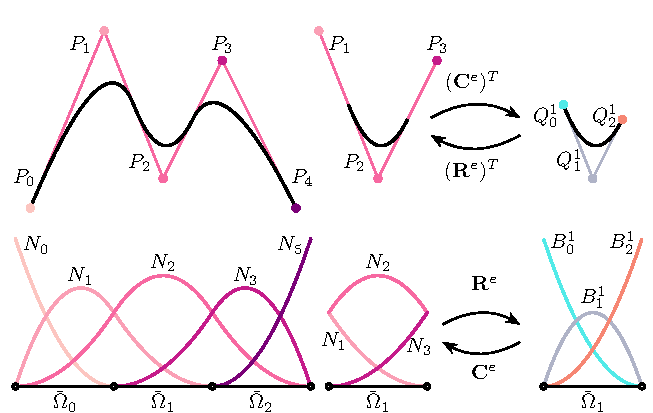
\includegraphics[width=.7\linewidth]{elements_global.pdf}
        \caption{}\label{fig:element_extraction_projection}
    \end{subfigure}
    \begin{subfigure}{\linewidth}
        \center
        \includestandalone[scale = .8]{bezier_extraction_demo}
        \caption{}\label{fig:bezier_extraction_process}
    \end{subfigure}
    \caption{Illustration of \Bezier extraction and projection in one dimension for a B-spline of degree 2 and knot vector $\left\{0,0,0,1/3/2/3,1,1,1\right\}$. (a) The element extraction and projection for the second element. (b) \Bezier extraction over the entire domain.}
\end{figure}

It is possible to view \Bezier projection as a global assembly procedure. The B-spline basis vector $\mathbf{N}$ of dimension $n_N$ can be represented by a set of Bernstein basis functions $\mathbf{B}$ of dimension $n_B$ defined on each element as
\begin{equation}
	\mathbf{N} = \mathbf{A}^T\mathbf{C}\mathbf{B},
\end{equation}
where $\mathbf{C}$ is a block diagonal matrix with \Bezier element extraction operators on the diagonal and the rectangular assembly operator $\mathbf{A}$ is the permutation matrix that maps local element degrees of freedom to global degrees of freedom. The assembly operator $\mathbf{A}$ satisfies the following properties:
\begin{itemize}
	\item Each row of $\mathbf{A}$ contains a single unity-valued entry; all other entries are zero.
	\item Each column of $\mathbf{A}$ contains at most $p+1$ unity-valued entries; all other entries are zero.
	\item Compact support. The non-zero entries can be associated to no more than $p+1$ consecutive elements.
	\item If we consider the column vectors $\mathbf{A}_i$ of $\mathbf{A}$, the space $\spn\left\{\mathbf{A}_i\right\}_{i=0}^{n_N-1}$ is an $n_N$ dimensional subspace of $\mathbb{R}^{n_B}$ and $\left\{\mathbf{A}_i\right\}_{i=0}^{n_N-1}$ are orthogonal, i.e.
	      \begin{equation}
		      \mathbf{A}_i\cdot\mathbf{A}_j\neq{}0\iff{i=j}.
	      \end{equation}
\end{itemize}

The \Bezier extraction process for the quadratic B-spline basis defined by the knot vector $\{0,0,0,1/3,2/3,1,1,1\}$ is shown in Fig.~\ref{fig:bezier_extraction_process}. The assembly operator $\mathbf{A}$ for this example is given by
\begin{equation}\label{eq:assembly_matrix}
	\mathbf{A} =
	\begin{blockarray}{cccccc}
		N_0 & N_1  & N_2  & N_3  & N_4 \\
		\begin{block}{[ccccc]c}
			1 & \hfsetfillcolor{hred!10}\hfsetbordercolor{hred}\tikzmarkin{a}(0.1,-0.1)(-0.1,0.35)0 & 0 & 0 & 0 & N_0^0 \\
			0 & 1 & 0 & 0 & 0 & N_1^0 \\
			0 & 0 & 1 & 0 & 0 & N_2^0 \\
			0 & 1 & 0 & 0 & 0 & N_0^1 \\
			0 & 0 & 1 & 0 & 0 & N_1^1 \\
			0 & 0 & 0\tikzmarkend{a} & 1 & 0 & N_2^1 \\
			0 & 0 & 1 & 0 & 0 & N_0^2 \\
			0 & 0 & 0 & 1 & 0 & N_1^2 \\
			0 & 0 & 0 & 0 & 1 & N_2^2 \\
		\end{block}
	\end{blockarray},
\end{equation}
where the highlighted submatrix is the restriction of $\mathbf{A}$ onto elements $\Omega_0$ and $\Omega_1$, and onto the B-spline basis functions $N_1$ and $N_2$.

\subsection{B\'ezier projection}
\label{sec:bproject}

B\'{e}zier projection can be viewed as the inverse of extraction~\cite{thomas_bezier_2015}. It defines an surjection that maps a space spanned by  piecewise Bernstein basis onto a space spanned by B-spline basis. B\'ezier projection uses an element reconstruction operator $\mathbf{R}^e\equiv(\mathbf{C}^e)^{-1}$ such that the global control point values, corresponding to those basis functions defined over the support of an element $e$, can be determined directly from \Bezier control values as
\begin{equation}
    \mathbf{P}^e=(\mathbf{R}^e)^T\mathbf{Q}^e
\end{equation}
where $\mathbf{Q}^e$ is any field in B\'ezier form. The action of the element reconstruction operator is depicted graphically in Figure~\ref{fig:element_extraction_projection}. For example, given any function $u \in L^2$, we can compute $\mathbf{Q}^e$ as
\begin{equation}
    \mathbf{Q}^e=(\mathbf{G}^e)^{-1}\mathbf{F}^e
    \label{eq:element-Qi}
\end{equation}
where $\mathbf{G}^e$ is the Gramian matrix corresponding to the Bernstein basis with components
\begin{align}
    {G}_{ij}^e & = \int_{\Omega^e} B^e_i B^e_j \, d\Omega =\langle{B^e_{i},B^e_{j}}\rangle_{\Omega^e}\label{eq:element_gramian}
\end{align}
and
\begin{align}
    {F}^e_i & =  \int_{\Omega^e} B^e_i u \, d\Omega = \langle{B^e_{i,},u}\rangle_{\Omega^e}.
\end{align}
Note that efficiency gains can be had at the expense of accuracy by instead performing the integration in the parametric domain of the element~\cite{thomas_bezier_2015}.

The element-wise projection produces one control value for each element in the support of the function.  These values must be combined in order to provide the final control value.  A core component of the B\'ezier projection algorithm is the definition of an appropriate averaging operation. The process of computing the weights is illustrated in Figure~\ref{fig:weights}. A weighted average of the values is computed using the weighting
\begin{equation}\label{eq:Bezier_weight}
    \omega_a^e=\dfrac{\int_{\Omega^e} N_{a}^e \, d\Omega}{\int_{\Omega^A} N_{A(e,a)} \, d\Omega}
\end{equation}
where $\Omega^e$ corresponds to the physical domain of element $e$, $A(e,a)$ is a mapping from a local nodal index $a$ defined over element $e$ to a corresponding global node index $A$, and $\Omega^A$ corresponds to the physical support of $N_A$. The final averaged global control point is then calculated as
\begin{equation}
    P_A=\sum_{\Omega^e\in \Omega^A } \omega_{A(e,a)} P_{A(e,a)}.
\end{equation}
B\'ezier projection onto NURBS functions can be defined in an analogous manner~\cite{thomas_bezier_2015}.

The individual steps comprising the \Bezier projection algorithm are
illustrated in Figure~\ref{fig:loc-proj-example} where
the curve defined by $\vec{f}(t)=\left( \frac{t}{3}
    \right)^{3/2}\vec{e}_1+\frac{1}{10}\sin (\pi t )\,\vec{e}_2$,
$t\in[0,3]$ is projected onto the quadratic B-spline basis defined by
the knot vector $\left\{0,0,0,\frac{1}{3},\frac{2}{3},1,1,1\right\}$. For this example,
the algorithm proceeds as follows:

\begin{description}

    \item{Step 1:} The function $\mathbf{f}$ is projected onto the Bernstein basis of each element. This results in a set of
          \Bezier coefficients that define an approximation to $\mathbf{f}$.
          The \Bezier coefficients are indicated in part (1) of Figure~\ref{fig:loc-proj-example} by
          square markers that have been colored to match the corresponding
          element. Each \Bezier segment is discontinuous.

    \item{Step 2:} The element reconstruction operator $\mathbf{R}^e$ is used to convert the
          \Bezier control points into spline control points associated with the
          basis function segments over each element.
          The new control points are marked with inverted triangles and
          again colored to indicate the element with which the control point is
          associated. The control points occur in clusters.
          The clusters of control points represent the contributions from
          multiple elements to a single spline basis function control point.

    \item{Step 3:} Each cluster of control points is averaged to obtain a
          single control point by weighting each point in the cluster according
          to the weighting given in (\ref{eq:Bezier_weight}). The resulting control
          points are shown as circles with the relative contribution from each
          element to each control point indicated by the colored fraction of the
          control point marker. Colors in Figures~\ref{fig:weights} and~\ref{fig:loc-proj-example} are coordinated
          to illustrate where the averaging weights come from and their values.
\end{description}

\begin{figure}[htb]
    \centering
    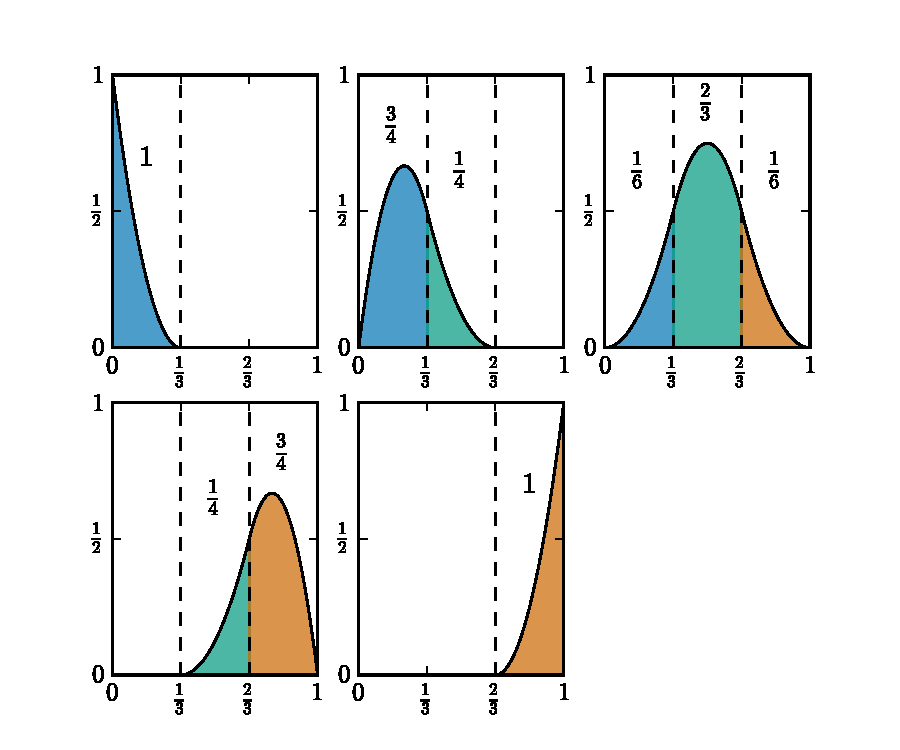
\includegraphics[width=5in]{weights.pdf}
    \caption{\label{fig:weights}Weights over each knot span associated
        with the basis function defined by the knot vector
        $[0,0,0,\frac{1}{3},\frac{2}{3},1,1,1]$.}
\end{figure}
\begin{figure}[htb]
    \centering
    \begin{tabular}{c p{4in} p{2in}}
        (0) & \raisebox{-.5\height}{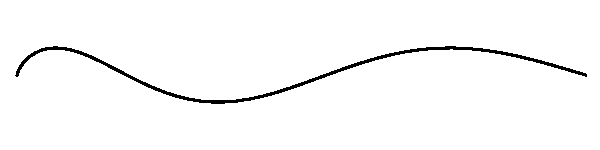
\includegraphics[width=4in]{local_proj_steps1.pdf}} & \begin{minipage}[t]{2in}Target function\end{minipage} \\
        (1) & \raisebox{-.5\height}{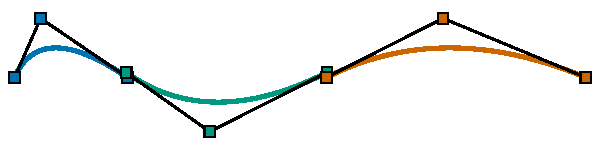
\includegraphics[width=4in]{local_proj_steps2.pdf}} & \begin{minipage}[t]{2in}Perform local projection to obtain \Bezier control points (represented by squares, colored to match elements)\end{minipage} \\
        (2) & \raisebox{-.5\height}{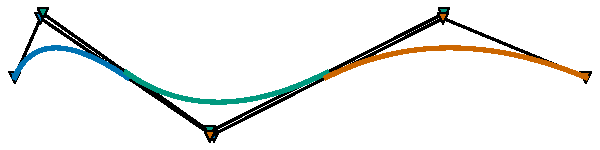
\includegraphics[width=4in]{local_proj_steps3.pdf}} & \begin{minipage}[t]{2in}Use element reconstruction operator to project \Bezier points to spline control points (represented by inverted triangles, colored to match elements)\end{minipage} \\
        (3) & \raisebox{-.5\height}{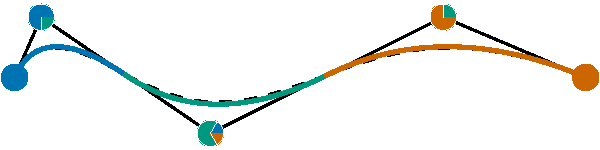
\includegraphics[width=4in]{local_proj_steps4.pdf}} & \begin{minipage}[t]{2in}Apply smoothing algorithm (contribution of each element to each control point shown by colored fraction)\end{minipage} \\
        (4) & \raisebox{-.5\height}{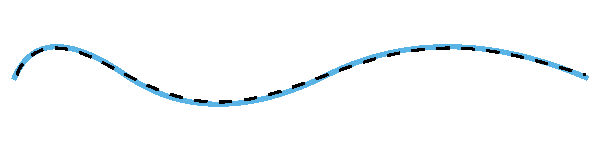
\includegraphics[width=4in]{local_proj_steps5.pdf}} & \begin{minipage}[t]{2in}Comparison of final function (light blue) and target function (dashed)\end{minipage}
    \end{tabular}
    \caption{\label{fig:loc-proj-example}Steps of \Bezier projection.}
\end{figure}

\section{Dual basis}\label{sec:dual_basis}
%%TODO: bezier dual basis function will be used for what?
In this section, we give a brief introduction to the concept of global and \Bezier dual basis functions. \Bezier dual basis functions will be used in Section to facilitate the solution of domain coupling problems in the dual mortar method. A dual basis is defined as a set of basis functions $\{\hat{N}_i\}_{i=1}^{n}$, which are dual to a corresponding set of primal basis functions $\{{N}_i\}_{i=1}^{n}$ in the sense that
\begin{equation}\label{eq:def:dual}
    \langle\hat{N}_i,N_j\rangle_\Omega:=\int_\Omega\hat{N}_iN_jd\Omega=\delta_{ij}, \quad\forall{}i,j\in\left[1,2,\dots,n\right],
\end{equation}
where $\delta_{ij}$ is the Kronecker delta.

\subsection{Global dual basis}

The global dual basis functions  $\{\hat{N}_i^G\}_{i=1}^{n}$ for a given set of primal basis function $\{{N}_i\}_{i=1}^{n}$ can be computed as
\begin{equation}
    \hat{N}_i^G=\sum_j G^{-1}_{ij}N_j,\label{eq:global_dual}
\end{equation}
where  $G^{-1}_{ij}$ are the components of the inverse of the Gramian matrix $\mathbf{G}$ with components $G_{ij}=\langle{N}_i,N_j\rangle_\Omega$.


In Isogeometric Analysis, we choose B-spline functions as the primal basis. One important property of B-spline functions is that they have compact support. This leads to sparse linear systems when these functions are used to define the trial and weighting function spaces in a Galerkin method. The global dual basis functions, however, do not have compact support and will result in dense linear systems when used as the weighting function space in a Galerkin method. Dual basis supports are shown in Figure~\ref{fig:bezier_extraction_illustration} where we have highlighted one B-spline function in Figure~\ref{fig:b-spline-func} and then shown the corresponding global dual basis function in Figure~\ref{fig:global_dual}.

\begin{figure}[ht]
    \center
    \begin{subfigure}{\linewidth}
        \center
        \includestandalone[scale=1]{basisfunctions}
        \caption{}\label{fig:b-spline-func}
    \end{subfigure}
    \begin{subfigure}{\linewidth}
        \center
        \includestandalone[scale=1]{dual_global_one}
        \caption{}\label{fig:global_dual}
    \end{subfigure}
    \begin{subfigure}{\linewidth}
        \center
        \includestandalone[scale=1]{bezier_dual_one}
        \caption{}\label{fig:bezier_dual}
    \end{subfigure}
    % or use \input{mytikz}
    \caption{A comparison of a B-spline basis function (a) with the corresponding global dual basis function (b) and the \Bezier dual basis function (c).}
    \label{fig:bezier_extraction_illustration}
\end{figure}

\subsection{\Bezier dual basis}

To maintain the sparsity of linear systems we will use \Bezier dual basis functions, which are computed locally and have compact support. These functions are computed using the \Bezier projection operator introduced in~\cite{thomas_bezier_2015}. The \Bezier dual basis has been shown to be effective in reducing volumetric and shear locking~\cite{MIAO2018273}, alleviating membrane locking in Kirchhoff-Love shells~\cite{greco2018reconstructed}, and as a dual mortaring strategy for elasticity problems~\cite{zou2018isogeometric}.

The construction of \Bezier dual basis functions leverages \Bezier extraction/projection~\cite{borden2011isogeometric, thomas2015bezier} and can be performed in several simple steps. For a given \Bezier element, $\Omega_e$, the element extraction operator $\mathbf{C}^e$ is computed. The element extraction operator maps a set of Bernstein polynomials $\{B_i\}_{i=1}^m$ defined over a \Bezier element, where $m$ depends on the polynomial degree of the \Bezier element in each parametric direction, into the set of global B-spline basis functions that have support over that element. The element reconstruction operator, $\mathbf{R}^e$, and the Gramian matrix, $\mathbf{G}^{e}$~\eqref{eq:element_gramian}, of the Bernstein polynomials defined over the element are then computed. The element extraction operator for the dual basis is then simply
\begin{equation}
    \hat{\mathbf{D}}^e=\text{diag}(\omega^e)\mathbf{R}^e\left[\mathbf{G}^{e}\right]^{-1}
\end{equation}
where $\text{diag}(\omega^e)$ is a diagonal matrix with the \Bezier projection weights~\eqref{eq:Bezier_weight} on the diagonal.

The restriction of a \Bezier dual basis functions $\hat{N}_i^B$ to $\Omega_e$ is then computed as
\begin{equation}
    \hat{N}^B_i\vert_{\Omega_e}=\sum_{j=1}^m\hat{D}^e_{ij}B_j.\label{eq:bezier-dual-basis}
\end{equation}
From this local definition of the dual basis over an element we have
\begin{equation}
    \int_{\Omega_e}\hat{N}^B_iN_jd\Omega=\omega^e_i\delta_{ij},
\end{equation}
and
\begin{equation}
    \A_e{} \int_{\Omega_e}\hat{N}^B_iN_jd\Omega=\delta_{ij},
\end{equation}
where $\A$ is the standard assembly operator \cite{Hug00} . The \Bezier dual basis of the B-spline basis function highlighted in Figure~\ref{fig:b-spline-func} is shown in Figure~\ref{fig:bezier_dual}. Note that the \Bezier dual basis function has the same compact support as the primal B-spline basis function.

\subsection{Rational dual basis functions}
If rational basis functions are used, the construction of the dual basis must be modified slightly. A rational dual basis must satisfy the biorthogonality requirement
\begin{align}
    \int_{\Omega} \bar{R}_A R_B \, d\Omega= \delta_{AB}.
\end{align}
A simple way to achieve biorthogonality is to define
\begin{align}
    \bar{R}_A & = W \bar{N}_A/w_A
\end{align}
where $W$ is the rational weight given in (\ref{eq:weight}). Now
\begin{align}
    \int_{\Omega} \bar{R}_A R_B \, d\Omega & = \int_{\Omega} \bar{N}_A N_B \, d\Omega = \delta_{AB}.
\end{align}

\begin{remark}
    The \Bezier dual basis functions define a quasi-interpolation operator $\mathcal{T}(f)=\sum_i \langle\hat{N}^B_i,f\rangle N_i$, which possesses the following properties:
    \begin{itemize}
        \item Optimal approximation: for $p^\text{th}$ order spline basis function and $f\in C^\infty$, the approximation error is given by~\cite{thomas_bezier_2015}
              \begin{equation}
                  \|\mathcal{T}(f)-f\|_{L^2}\leq Ch^{p+1}\|f\|_{H^{p+1}}.
              \end{equation}
        \item Boundary interpolation: for two sets of $p^\text{th}$ order spline basis functions $\{{N^s_i}\}_{i=1}^{n_s}$ and $\{{N^m_i}\}_{i=1}^{n_m}$ defined on $\left[{0,L}\right]$, if the first and last elements of $s$ are subsets of the first and last elements of $m$, then
              \begin{equation}
                  \mathcal{T}^s(f^m)(0)=f^m(0)\;\text{ and }\;\mathcal{T}^s(f^m)(L)=f^m(L),\quad\forall f^m\in\spn\{{N^m_i}\}_{i=1}^{n_m}.\label{eq:boundary_interpolation}
              \end{equation}
    \end{itemize}
    The second property is critical for the coercivity of the biharmonic problem on multi-patch domains.
\end{remark}